\chapter{Using the library well}
\label{ch:practice}

This chapter collects the practical consequences of everything above.

\section{Rules of thumb for cost}

\begin{itemize}
  \item \textbf{Multiplication is the unit of cost.} Division of similar-sized numbers costs a few
        multiplications; decimal conversion of an $n$-limb number costs about $\log_2 n$
        multiplications of decreasing size. The cost of a square depends on whether the
        transform reuses the first operand's spectrum (\cref{sec:nttreuse}).
  \item \textbf{Doubling the size} roughly quadruples the time below about 25 limbs, triples it in
        the Karatsuba range, and usually a little more than doubles it within the single-transform
        NTT range. Above that range the number of block pairs also determines the cost.
  \item \textbf{Lopsided products are cheap.} $10 \times 100\,000$ limbs is a million limb products,
        no worse than adding the long number to itself ten times.
  \item \textbf{Transform boundaries matter for latency.} For balanced threaded
        products, increasing each operand from 10 million to 11 million digits
        doubles the transform length. The boundary is near 10.10 million digits
        (\cref{sec:trunc}).
\end{itemize}

Warm operation times on the Apple M1 Max, in milliseconds, on revision \code{9d3f1d4}.

\begin{center}
\small
\begin{tabular}{lrrr}
\toprule
operation (decimal digits) & BigMath 1 thread & BigMath default & GMP 1 thread \\
\midrule
multiply $10^4 \times 10^4$ & 0.05058\,ms & 0.03596\,ms & 0.02796\,ms \\
multiply $10^6 \times 10^6$ & 9.542\,ms & 2.948\,ms & 9.133\,ms \\
multiply $10^7 \times 10^7$ & 111.1\,ms & 16.52\,ms & 201.9\,ms \\
multiply $50\,{\rm M} \times 50\,{\rm M}$ & 634.4\,ms & 172.2\,ms & 660\,ms \\
multiply $100\,{\rm M} \times 100\,{\rm M}$ & 1\,372\,ms & 388.4\,ms & 1\,392\,ms \\
multiply $200\,{\rm M} \times 200\,{\rm M}$ & 2\,885\,ms & 723.8\,ms & 2\,852\,ms \\
divide $10^7 \div (2\cdot 10^6)$ (quotient) & 157.7\,ms & 53.45\,ms & 145.9\,ms \\
parse $2\cdot10^7$ digits & 880.2\,ms & 159.4\,ms & 806.6\,ms \\
print $2\cdot10^7$ digits & 2\,462\,ms & 503.9\,ms & 2\,144\,ms \\
\bottomrule
\end{tabular}

\smallskip
{\footnotesize The two BigMath builds used the same operands and GMP reference.
The default build uses up to eight threads. The full benchmark records one warm
observation for most large inputs. Data and repetition counts are in \file{BENCHMARK.md}.}
\end{center}

\begin{figure}[ht]
\centering
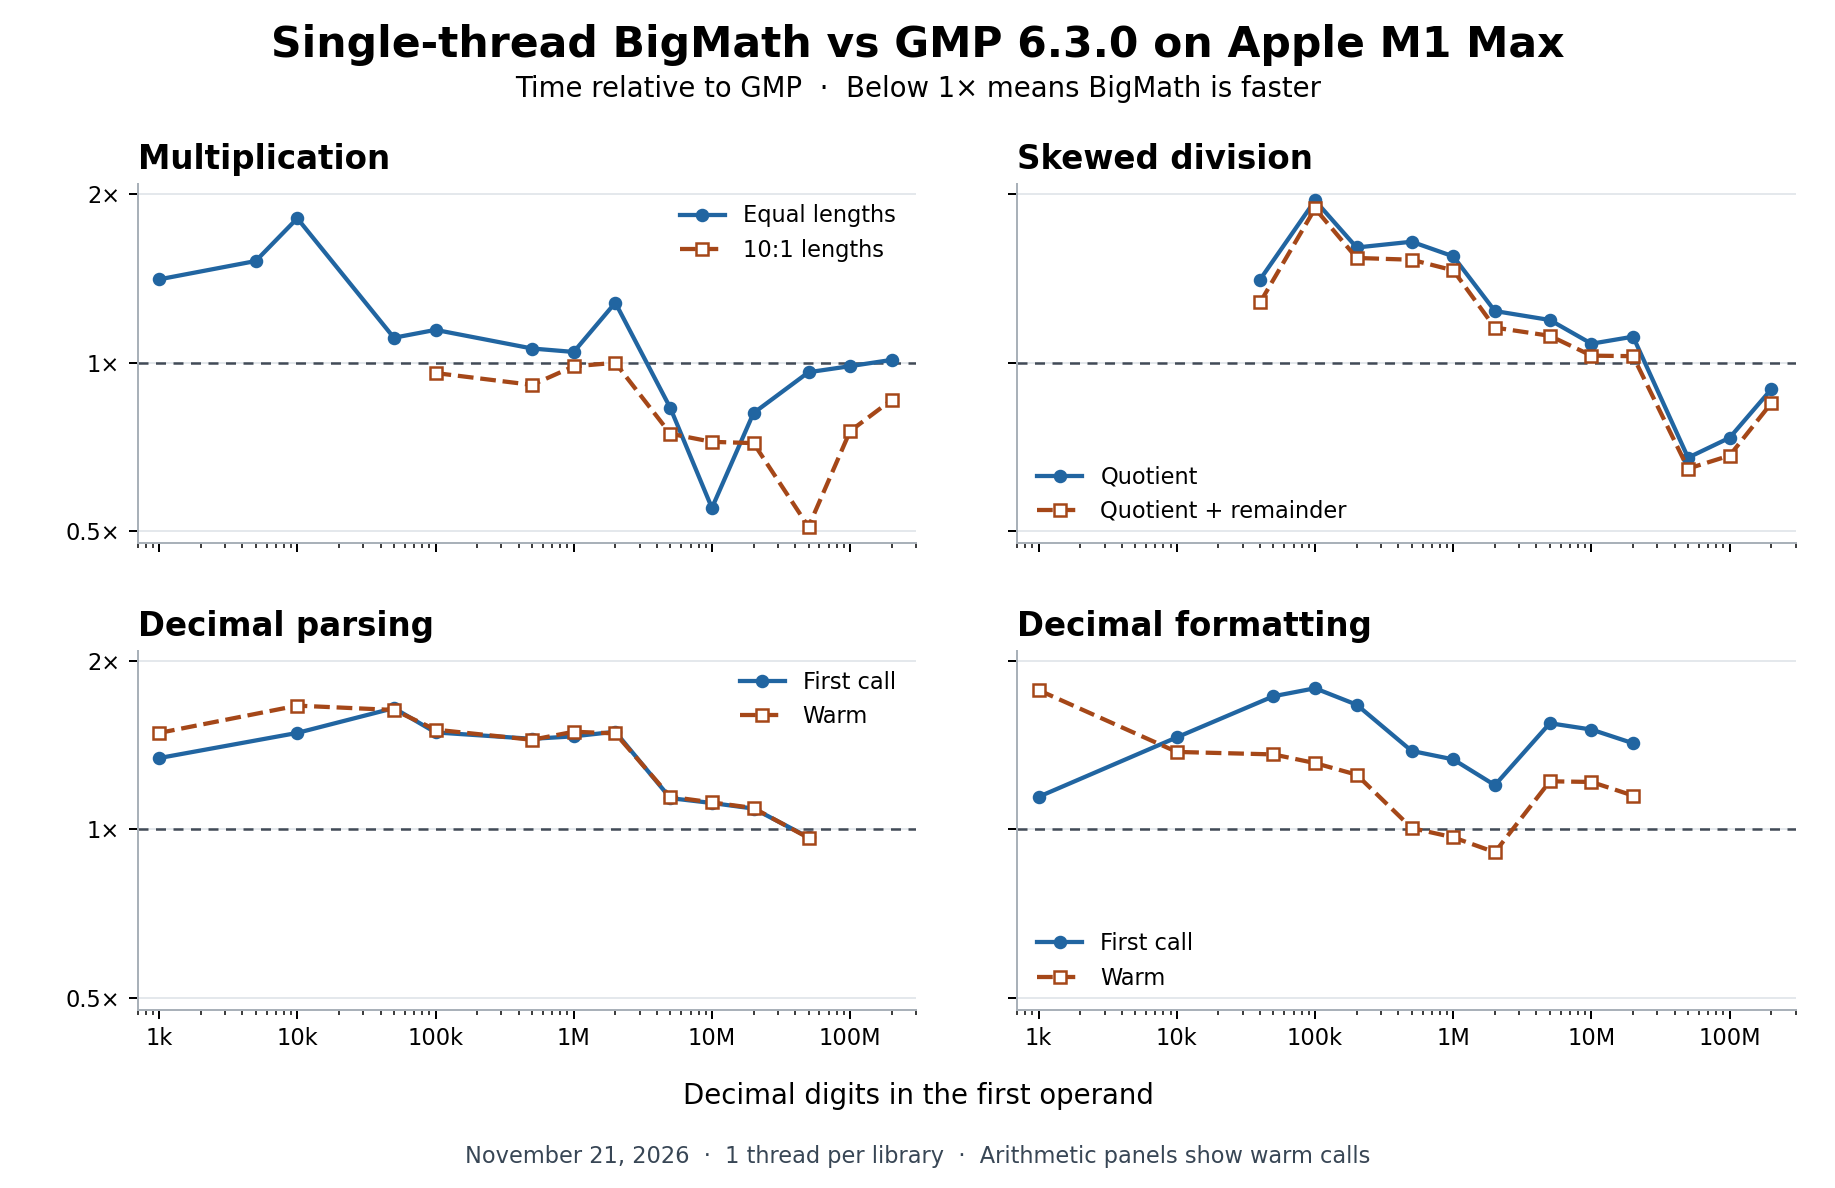
\includegraphics[width=\textwidth]{../images/bigmath_vs_gmp_single_thread.png}
\caption{Single-threaded BigMath time divided by single-threaded GMP time (below 1 means BigMath
was faster). From \file{docs/images/}, generated from the November 2026 benchmark run.}
\end{figure}

\begin{figure}[ht]
\centering
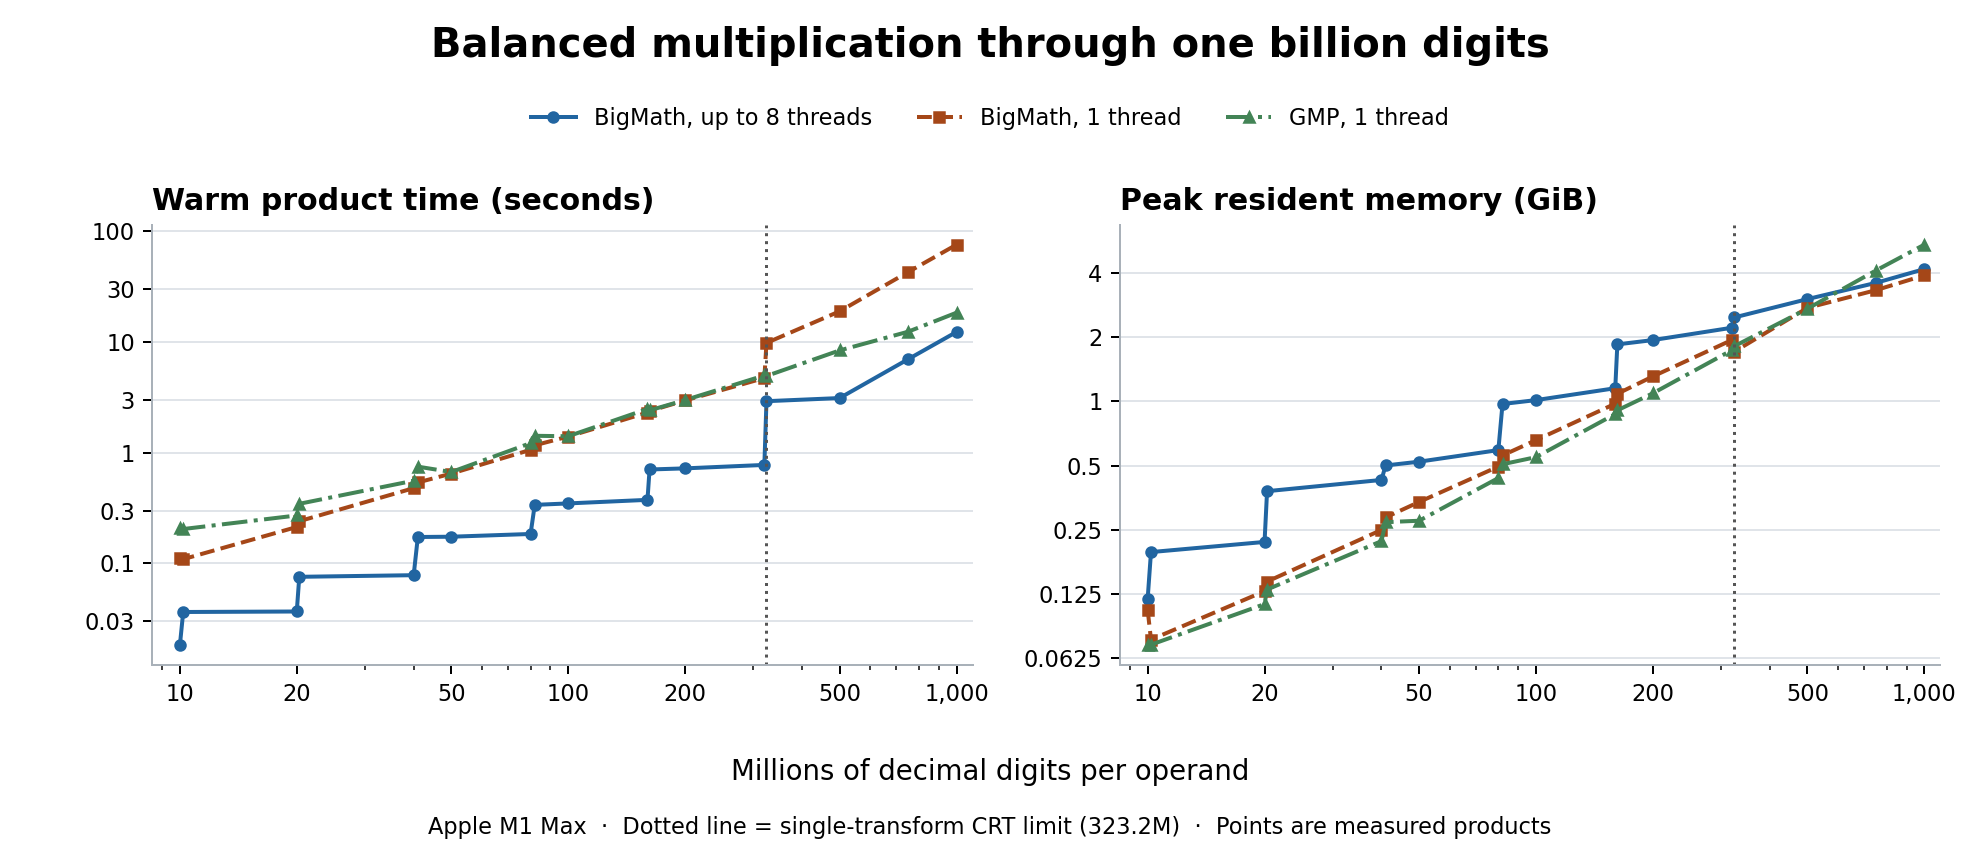
\includegraphics[width=\textwidth]{../images/bigmath_vs_gmp_large_products.png}
\caption{Fresh-process measurements through one billion decimal digits per operand.
The dotted line marks the largest single CRT transform. Products above it accumulate
multiple block products. Each point reports one warm multiplication and the process
peak through that call.}
\end{figure}

\section{Choosing the right call}

\begin{center}
\small
\renewcommand{\arraystretch}{1.25}
\begin{tabularx}{\textwidth}{lX}
\toprule
you want & use \\
\midrule
$a \times b$ & \code{a * b}. The dispatcher picks the method. \\
$a^2$ & \code{a * a} with the \emph{same object} on both sides: the library notices and squares. \\
many products with one fixed large factor & \code{PrepareMultiplication(a, maxOtherLimbs)} (\cref{ch:ntt}). \\
quotient only & \code{a / b}; much faster than \code{DivideAndRemainder} when the quotient is
               shorter than the divisor (\cref{sec:toplimbs}). \\
quotient and remainder & \code{DivideAndRemainder(a, b)}, one division for both. \\
many divisions by one divisor & \code{CacheDivision(b)} (\cref{sec:cached}). \\
division by a small constant & the \code{uint64\_t} overloads: \code{a / 10}, \code{a \% 10}. \\
text in / out & \code{BigIntegerBuilder::From(str)}, \code{ToString(x)}; the second call of a similar size is much faster than the first. \\
\bottomrule
\end{tabularx}
\end{center}

\section{Build options that change algorithms}

\begin{center}
\small
\begin{tabularx}{\textwidth}{lX}
\toprule
option & effect \\
\midrule
\code{-DBIGMATH\_USE\_THREADS=0} & no thread pool, no pthread dependency; every pool-dependent
                                   choice uses its ``cold'' threshold. \\
\code{-DBIGMATH\_MAX\_THREADS=N} & cap the pool at $N$ threads (default 8). \\
\code{-DBIGMATH\_POOL\_SPIN\_US=0} & idle workers sleep immediately: least idle CPU, slower
                                   bursts. \\
\code{-DBIGMATH\_NTT\_CRT=0} & single-prime (Goldilocks) NTT instead of three primes. Slower;
                              for comparison or unusual targets. \\
\code{-DBIGMATH\_NEON=0} & disable the ARM vector butterflies. \\
\code{-DBIGMATH\_LIMB\_64=0} & the legacy 32-bit-values-in-64-bit-slots layout; roughly 2$\times$
                              slower; for comparison. \\
any \code{-DBIGMATH\_*\_THRESHOLD=}$n$ & move a switch point (\cref{app:ref}). \\
\bottomrule
\end{tabularx}
\end{center}

Threshold overrides must be in effect when the \emph{library} is compiled (pass them through
\code{CMAKE\_CXX\_FLAGS}), because the dispatchers are compiled into \file{libbigmath.a}.

\section{Tuning for your machine}

The shipped thresholds were measured on an Apple M1 Max. On a different processor the crossovers
move, usually by tens of percent, not by factors. To measure your own:

\begin{lstlisting}[language=bash]
cmake -S . -B build -DCMAKE_BUILD_TYPE=Release
cmake --build build --target dispatch_tuner -j
./build/dispatch_tuner --full --emit-header \
    include/biginteger/build/platform/<os>-<arch>-<compiler>.h
\end{lstlisting}

The generated header is picked up automatically for that OS, architecture and compiler
(\file{docs/PLATFORM\_TUNING.md}). Precedence: command-line \code{-D} first, then the platform
profile, then the defaults in \file{DispatchThresholds.h}.

\section{Checking correctness after a change}

All algorithms are cross-checked against each other:

\begin{itemize}
  \item \code{mult\_correctness} multiplies with every method and compares limb for limb against
        schoolbook;
  \item \code{div\_correctness} runs every division algorithm, compares against reference
        implementations, and checks $q \cdot b + r = a$ and $0 \le r < b$ on every result;
  \item unit tests pin details such as the reciprocal's error bound, the zero-fallback guarantee
        of Newton division, and NTT layers against a plain radix-2 transform.
\end{itemize}

Run \code{ctest --output-on-failure} in the build directory after changing a threshold or an
algorithm. Passing means the new path agrees with an independent reference path, not just that it
ran.
